\section{Spectral descriptors, design sensitivities, and robust paths}
\label{sec:design-descriptors}

The transformations themselves generate machine descriptors.  In whitened
coordinates,
\begin{equation}
 \widetilde{matr H}=\matr R^{-1/2}\matr H\matr R^{-1/2}
\end{equation}
has eigenvalues
\begin{equation}
 \operatorname{eig}(\widetilde{matr H})=
 \{-\kappa/2,0,\kappa/2\}.
 \label{eq:whitened-torque-spectrum}
\end{equation}
Thus
\begin{equation}
 \boxed{\lambda_{\max}(\widetilde{matr H})
 =\frac{M_{\max}^{(U\,\mathrm{free})}}{P_{\mathrm{Cu},\max}}
 =\frac{\kappa}{2}}
 \label{eq:spectral-capability}
\end{equation}
is exactly torque per watt of optimally allocated copper loss in the linear
model, not merely a heuristic index.  Its eigenvector is the balanced
\((z_\psi,z_q)\) current direction.

Likewise,
\begin{equation}
 \widetilde{matr Q}=\matr R^{-1/2}\matr Q_U\matr R^{-1/2}
\end{equation}
has units \(\mathrm{V^2/W}=\Omega\).  Its Rayleigh quotient is squared voltage
per copper loss, and its two positive eigenvalues give the principal voltage
prices.  In the EESM the third eigenvalue is zero because the stator-voltage
map has a null direction.  A useful fingerprint therefore reports the torque
spectrum, the positive voltage spectrum, and several support values
\begin{equation}
 h(\mu;\boldsymbol\theta)=
 \lambda_{\max}(\widetilde{matr H}-\mu\widetilde{matr Q}).
 \label{eq:spectral-support-fingerprint}
\end{equation}
No fixed handful of eigenvalues completely determines the joint eigenvector
geometry, but these quantities cheaply distinguish machines that share the
same loss-only optimum and differ under voltage.

\subsection{Sensitivities that retain physical meaning}

Let \(C=\kappa/2=(k_T/2)r_M\), and define mechanism weights
\begin{equation}
 w_x=\frac{x_M^2}{r_M^2},\qquad w_y=\frac{y_M^2}{r_M^2},
 \qquad w_x+w_y=1.
\end{equation}
For nonzero coordinates the logarithmic sensitivities are
\begin{align}
 \frac{\partial\ln C}{\partial\ln|\Delta L|}&=w_x,&
 \frac{\partial\ln C}{\partial\ln L_{\mathrm{exc}}}&=w_y,
 \label{eq:capability-elasticity-positive}\\
 \frac{\partial\ln C}{\partial\ln R_s}&=-w_x-\frac12w_y,&
 \frac{\partial\ln C}{\partial\ln R_{\mathrm{exc}}}&=-\frac12w_y,&
 \frac{\partial\ln C}{\partial\ln p}&=1.
 \label{eq:capability-elasticity-cost}
\end{align}
These formulas say more than ``lower resistance is better.''  A
reluctance-dominated machine receives nearly unit elasticity from saliency and
stator resistance, while an excitation-dominated machine receives unit
elasticity from coupling inductance but only half-order penalties from each
resistance.  In the \((x_M,y_M)\) plane the gradient
\(\nabla r_M=(x_M,y_M)/r_M\) is normal to the capability circle, so it points
along the locally fastest capability improvement.  Tangential parameter
changes alter the mechanism mix without changing first-order loss-only
capability.

These are electromagnetic partial derivatives, not independent geometry
knobs.  A physical change can move several entries of \(\boldsymbol\theta\)
at once.  If \(\boldsymbol\theta=\mathcal M(\vect g)\), the relevant geometry
sensitivity is the chain rule
\begin{equation}
 \nabla_{\vect g}C=
 \left(\frac{\partial\mathcal M}{\partial\vect g}\right)^{\mathsf T}
 \nabla_{\boldsymbol\theta}C.
 \label{eq:geometry-chain-rule}
\end{equation}

\subsection{A design is a parameter path, not a nominal point}

Temperature, frequency, and saturation produce a family
\(\boldsymbol\theta(\xi)\), \(\xi\in\gls{sym:operatingdomain}\).  Robust
feasibility is
\begin{equation}
 \boxed{M_{\max}(\boldsymbol\theta(\xi))
 \geq M_{\mathrm{req}}(\xi)\quad\forall\xi\in\mathcal O.}
 \label{eq:robust-design-path}
\end{equation}
In the analytic loss-only map, the entire path must remain outside the
requirement circle.  With voltage, evaluate the minimum margin of
\cref{eq:voltage-design-levelset} over the operating and uncertainty grid.
Resistance growth with temperature moves an EESM inward; saturation changes
both \(x_M\) and \(y_M\); PM temperature also moves a PSM's normalized flux
and characteristic-current ratio.  A nominal point with no clearance is not a
robust design.

\begin{figure}[tb]
\centering
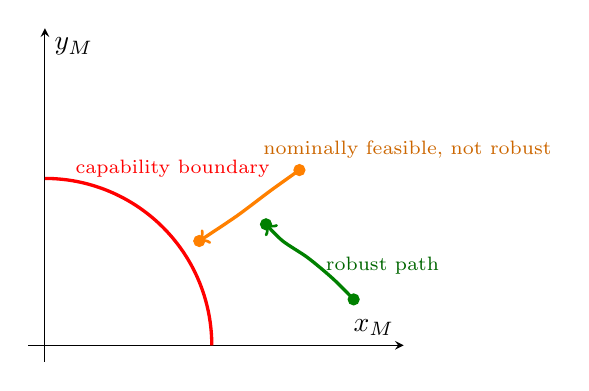
\begin{tikzpicture}
\begin{axis}[
 width=.72\linewidth,height=.48\linewidth,axis equal image,
 xmin=-.2,xmax=4.3,ymin=-.2,ymax=3.8,
 xlabel={$x_M$},ylabel={$y_M$},ticks=none,axis lines=middle,clip=false]
 \addplot[domain=0:90,samples=100,red,very thick] ({2*cos(x)},{2*sin(x)});
 \addplot[green!50!black,very thick,->,smooth]
  coordinates {(3.7,.55) (3.45,.8) (3.15,1.05) (2.85,1.25) (2.65,1.45)};
 \addplot[orange,very thick,->,smooth]
  coordinates {(3.05,2.1) (2.7,1.85) (2.3,1.55) (1.85,1.25)};
 \addplot[only marks,mark=*,green!50!black] coordinates {(3.7,.55) (2.65,1.45)};
 \addplot[only marks,mark=*,orange] coordinates {(3.05,2.1) (1.85,1.25)};
 \node[green!40!black,anchor=west,font=\scriptsize] at (axis cs:3.25,.95)
   {robust path};
 \node[orange!80!black,anchor=west,font=\scriptsize] at (axis cs:2.5,2.35)
   {nominally feasible, not robust};
 \node[red,anchor=south west,font=\scriptsize] at (axis cs:.25,1.9)
   {capability boundary};
\end{axis}
\end{tikzpicture}
\caption{Robust design is a path-containment requirement.  The green
temperature/saturation path remains feasible; the orange path crosses the
capability boundary although its nominal point is acceptable.}
\label{fig:robust-path}
\end{figure}



For nonlinear flux maps, the global circles are no longer exact.  A useful
extension is local: compute the differential torque matrix, local loss metric,
and local voltage Jacobian at each operating point, then track their spectral
descriptors.  The robust test uses the original nonlinear residuals and the
minimum local margin.  This preserves the interpretation of torque-producing,
torque-neutral, and voltage-expensive directions without pretending that one
constant inductance matrix describes the whole envelope.

